\documentclass{article}
\usepackage[utf8]{inputenc}
\usepackage[portuguese]{babel}
\usepackage[a4paper, total={7in, 9in}]{geometry}
\usepackage{graphicx}
\usepackage{float}
\usepackage{verbatim}
\usepackage{fancyvrb}
\usepackage[bottom]{footmisc}
\usepackage[style=numeric]{biblatex}
\usepackage{hyperref}
\usepackage{mathtools}
\usepackage[title]{appendix}
\usepackage{xcolor}
\usepackage{minted}
\usepackage{csquotes}
\usepackage{framed}

\addbibresource{references.bib}

\begin{document}

{
\center
\begin{figure}[H]
        \centering
        
\includegraphics[width=3cm]{Pictures/UM_EENG.jpg}
\end{figure}
\textsc{\Large Universidade do Minho} \\ [0.5cm]
\textsc{\Large Mestrado em Engenharia Informática} \\ [0.5cm]
\textsc{\large Processamento e Representação de Conhecimento} \\ [0.5cm]

{\LARGE \bfseries Musike - Music Linked} \\[0.5cm]

\begin{tabular}{c} 
    José Carlos Lima Martins \\
    A78821 \\
\end{tabular} \\[0.5cm]

\today \\[1cm]
}

\section{Introdução}

ENTREGA:\\
27 de Maio\\

\section{Contextualização}

O trabalho a desenvolver passa por escolher uma área/tema de trabalho. A partir desse tema, criar/construir/limpar/extrair um dataset sobre o tema e que esteja disponível na LOD (\textit{Linked Open Data}). Este dataset em Turtle (\textit{Terse RDF Triple Language}) será armazenado em \textit{GraphDB}, onde será possível aceder/realizar \textit{queries} ao dataset localmente.

De seguida, será criado um website/app web de forma a explorar o dataset anteriormente criado. Este website deve possuir autenticação, usando para isso o \textit{MongoDB}.

\section{Tema escolhido - \textbf{Musike}} \label{tema}

O \textbf{Musike}, abreviatura de \textit{Music Linked}, consiste num website com a informação de artistas, bem como, das suas músicas e dos seus albuns. Em termos de informação a apresentar, pretendesse o seguinte:
\begin{itemize}
    \item Artista
        \begin{itemize}
            \item nome
            \item alias
            \item tipo de artista (Grupo, Pessoa, etc)
            \item data de nascimento/inicio
            \item data de falecimento/fim
            \item sexo (não é aplicável a todos os tipos de artista)
            \item nacionalidade (obtido através da área)
            \item descrição
            \item urls para página pessoal, redes sociais, etc
            \item classificação dos utilizadores do website (média das classificações das músicas)
            \item soma das visualizações das várias músicas
        \end{itemize}
    \item Album
        \begin{itemize}
            \item título
            \item data do primeiro release
            \item artista(s)
            \item descrição
            \item músicas do album
            \item tipos (tags) do album (clássica, rock, etc)
            \item urls sobre o album
            \item classificação dos utilizadores do website (média das classificações das músicas)
            \item soma das visualizações das várias músicas
        \end{itemize}
    \item Música
        \begin{itemize}
            \item título
            \item artista(s)
            \item duração
            \item descrição
            \item língua(s)
            \item tipos (tags) da música (clássica, rock, etc)
            \item urls sobre a música
            \item classificação dos utilizadores do website
            \item número de vezes ouvida pelos utilizadores do website
        \end{itemize}
    \item Área
        \begin{itemize}
            \item nome
            \item tipo (país, cidade, etc)
            \item alias
            \item data de criação
            \item data de extinção
            \item descrição
            \item urls sobre a área
            \item relações com outas áreas, pois uma área pode ser parte de outra e, vice-versa, uma área pode incluir várias áreas
        \end{itemize}
\end{itemize}

Para além disso, para cada música o objetivo é ter na sua página o vídeo presente no \textit{YouTube} bem como a letra da música. Com isto, pretendesse que por cada visualização do vídeo se conte que a música foi ouvida uma vez.

Por outro lado, o website deve permitir aos utilizadores escolher as músicas e albuns que mais gosta, bem como, puder criar playlists.

Cada utilizador deve ter acesso às suas estatísticas, onde deve estar presente as músicas que o utilizador ouve mais, os artistas que ouve mais e os albuns que ouve mais.

Por fim, apresentar estatísticas gerais do website entre as quais:
\begin{itemize}
    \item músicas mais ouvidas pelos utilizadores
    \item artistas mais ouvidos pelos utilizadores
    \item tipos de músicas (tags) mais ouvidos pelos utilizadores
    \item albuns mais ouvidos pelos utilizadores
    \item países com mais artistas
    \item países com mais músicas
    \item países com mais albuns
    \item países mais ``ouvidos'' pelos utilizadores
\end{itemize}

De forma adicional, seria interessante dar sugestões ao utilizador de músicas a ouvir a partir das estatísticas do utilizador.

\section{Ontologia baseada no \textit{MusicBrainz}} \label{ontologia}

Para o tema escolhido é necessário um dataset que possua a informação de albuns, artistas, músicas e áreas. Como tal foi escolhido o dataset JSON do \textit{MusicBrainz}.

A partir deste dataset bem como das características do tema escolhido, foi construído a estrutura da ontologia e posteriormente foi povoada com a informação presente no dataset (JSON).

\subsection{Parte Estrutural da Ontologia}

O primeiro passo foi a construção da estrutura ontologia baseada no dataset JSON do \textit{MusicBrainz}~\cite{mbSchema}. O desenho da estrutura pode ser visualizado de seguida:

\begin{figure}[H]
    \centering
    \includegraphics[width=15cm]{Pictures/ontologySctructure.png}
    \caption{Estrutura da ontologia, imagem obtida através de \protect\href{http://www.visualdataweb.de/webvowl/}{WebVOWL}}
\end{figure}

As classes principais da ontologia são \textit{Artist}, \textit{Recording}, \textit{Album} e \textit{Area} que representam respetivamente Artista, Música, Album e Área. Uma classe também importante mas secundária, é a classe \textit{URL} que representa URL's. Por forma a organizar melhor as propriedades, visto que as subclasses herdam as propriedades/relações das superclasses, foram criadas as superclasses \textit{Entity}, \textit{MusicEntity} e \textit{TimeLimitedEntity}. \textit{MusicEntity} inclui as subclasses \textit{Recording} e \textit{Album} devido às duas possuírem a propriedade \textit{title}. Por outro lado, \textit{TimeLimitedEntity} tem como subclasses \textit{Artist} e \textit{Area}, visto que estas duas classes possuem uma data de inicio e de fim. Já a classe \textit{Entity} inclui as subclasses \textit{MusicEntity} e \textit{TimeLimitedEntity}, ou seja, é a superclasse das quatro principais classes, até porque estas quatro classes possuem as propriedades \textit{about} e \textit{disambiguation}.

Quanto às propriedades/relações, a ontologia apresenta as seguintes:
\begin{itemize}
    \item Propriedades (\textit{Data Properties})
    \begin{itemize}
        \item Classe \textbf{\textit{Entity}}
        \begin{itemize}
            \item \textbf{\textit{about}}: Descrição do elemento
            \item \textbf{\textit{disambiguation}}: Forma de desambiguar entre elementos com o mesmo nome
        \end{itemize}
        \item Classe \textbf{\textit{URL}}
        \begin{itemize}
            \item \textbf{\textit{label}}: o nome do website a que se refere o URL (exe: wikipédia)
            \item \textbf{\textit{value}}: URL propriamente dito
        \end{itemize}
        \item Classe \textbf{\textit{TimeLimitedEntity}}
        \begin{itemize}
            \item \textbf{\textit{name}}: Nome do elemento
            \item \textbf{\textit{alias}}: nomes alternativos e nomes com erros ortográficos, permitindo uma melhor busca quando o utilizador introduz o nome com erros 
            \item \textbf{\textit{type}}: Tipo do elemento (em \textit{Area}: district, contry, city, etc, já em \textit{Artist}: person, group, choir, etc)
            \item \textbf{\textit{beginDate}}: Data de inicio
            \item \textbf{\textit{endDate}}: Data de fim
        \end{itemize}
        \item Classe \textbf{\textit{MusicEntity}}
        \begin{itemize}
            \item \textbf{\textit{title}}: Título
        \end{itemize}
        \item Classe \textbf{\textit{Album}}
        \begin{itemize}
            \item \textbf{\textit{firstReleaseDate}}: Data da primeira ``release'' do Album
        \end{itemize}
        \item Classe \textbf{\textit{Recording}}
        \begin{itemize}
            \item \textbf{\textit{duration}}: Duração da música
            \item \textbf{\textit{language}}: Língua da música
            \item \textbf{\textit{tag}}: Tags (tipos) da música
        \end{itemize}
        \item Classe \textbf{\textit{Artist}}
        \begin{itemize}
            \item \textbf{\textit{gender}}: Género do artista
            \item \textbf{\textit{sortName}}: Nome de modo a ordenar o artista numa lista
        \end{itemize}
    \end{itemize}
    \item Relações (\textit{Object Properties})
    \begin{itemize}
        \item \textbf{\textit{from}}: De \textit{Arist} para \textit{Area}, indica que um artista é da área
        \item \textbf{\textit{hasURL}}: De \textit{Entity} para \textit{URL}, indica que uma entidade tem o URL
        \item \textbf{\textit{hasPart}}: De \textit{Area} para \textit{Area}, indica que uma área inclui a outra
        \item \textbf{\textit{partOf}}: Inverso de \textit{hasPart}, indica que uma área é parte de outra
        \item \textbf{\textit{artistCredit}}: De \textit{Recording} para \textit{Artist}, indica que a música tem como crédito o artista
        \item \textbf{\textit{hasCreditIn}}: Inverso de \textit{artistCredit}, indica que um artista tem crédito na música
        \item \textbf{\textit{hasTrack}}: De \textit{Album} para \textit{Recording}, indica que um album tem a música
        \item \textbf{\textit{trackIn}}: Inverso de \textit{hasTrack}, indica que uma música pertence a um album
    \end{itemize}
\end{itemize}

É importante voltar a referir que as subclasses herdam as propriedades das superclasses.

\subsection{De JSON para Turtle - Povoamento da Ontologia}

Com a estrutura da ontologia e com uma ideia da informação necessária, foi então usado um dataset (\url{http://ftp.musicbrainz.org/pub/musicbrainz/data/json-dumps/20190403-001001/}) para popular a ontologia. Este dataset é proveniente do \textbf{MusicBrainz} estando o mesmo em JSON. O seu timestamp é de 2019-04-03, portanto um dataset bastante recente possuindo cerca de 240GB de tamanho. Visto o mesmo estar em JSON é necessário então convertê-lo para Turtle.

Num primeiro passo, percorresse os ficheiros JSON (que em cada linha possui um elemento de tipo igual ao nome do ficheiro a percorrer) com os conversores criados em \textit{Node.js}. Foi criado um conversor por ficheiro a converter. Apresentam se os seguintes conversores, que para cada linha do ficheiro converte a informação para (origem $\to$ destino)~\cite{mbSchema,mbRels}:
\begin{itemize}
    \item Conversor para area.json (\textit{jsonTOturtle/area.js})~\cite{mbAr}:
        \begin{itemize}
            \item \textit{id} $\to$ ``area\_'' + \textit{id} de forma a identificar o indivíduo
            \item \textit{name} $\to$ \textit{data property} \textit{\textbf{name}}
            \item \textit{type} $\to$ \textit{data property} \textit{\textbf{type}}
            \item \textit{aliases} (lista em que de cada elemento usasse o \textit{name} e o \textit{locale}) $\to$ \textit{data property} \textit{\textbf{alias}} (um por elemento da lista no seguinte formato: ``\textit{name}(\textit{locale})'')
            \item \textit{life-span.begin} $\to$ \textit{data property} \textit{\textbf{beginDate}}
            \item \textit{life-span.end} $\to$ \textit{data property} \textit{\textbf{endDate}}
            \item \textit{annotation} $\to$ \textit{data property} \textit{\textbf{about}}
            \item \textit{disambiguation} $\to$ \textit{data property} \textit{\textbf{disambiguation}}
            \item \textit{relations} (lista) em que os elementos que possuírem:
                \begin{itemize}
                    \item \textit{type} igual a ``part of'' ou item \textit{area}: são transformados em relações entre indivíduos áreas usando \textit{area.id} para saber qual o id da área destino; para além disso, observasse a \textit{direction} por forma a saber a direção da relação $\to$ \textit{object property} \textit{\textbf{partOf}} (\textit{direction} ``backward'') ou \textit{\textbf{hasPart}} (\textit{direction} ``forward'')
                    \item item \textit{url}: guardasse o \textit{url.id} (identificador do url: ``url\_'' + \textit{url.id}), \textit{type} (\textit{\textbf{label}} de URL) e \textit{url.resource} (\textit{\textbf{value}} de URL) por forma a posterior criação do indivíduo URL e usasse \textit{url.id} para criar a relação entre area e URL a ser criado $\to$ \textit{object property} \textit{\textbf{hasURL}}
                \end{itemize}
        \end{itemize}
    \item Conversor para artist.json (\textit{jsonTOturtle/artist.js})~\cite{mbArt}:
        \begin{itemize}
            \item \textit{id} $\to$ ``artist\_'' + \textit{id} de forma a identificar o indivíduo
            \item \textit{area.id} $\to$ \textit{object property} \textit{\textbf{from}}
            \item \textit{name} $\to$ \textit{data property} \textit{\textbf{name}}
            \item \textit{type} $\to$ \textit{data property} \textit{\textbf{type}}
            \item \textit{aliases} (lista em que de cada elemento usasse o \textit{name} e o \textit{locale}) $\to$ \textit{data property} \textit{\textbf{alias}} (um por elemento da lista no seguinte formato: ``\textit{name}(\textit{locale})'')
            \item \textit{life-span.begin} $\to$ \textit{data property} \textit{\textbf{beginDate}}
            \item \textit{life-span.end} $\to$ \textit{data property} \textit{\textbf{endDate}}
            \item \textit{annotation} $\to$ \textit{data property} \textit{\textbf{about}}
            \item \textit{disambiguation} $\to$ \textit{data property} \textit{\textbf{disambiguation}}
            \item \textit{sort-name} $\to$ \textit{data property} \textit{\textbf{sortName}}
            \item \textit{gender} $\to$ \textit{data property} \textit{\textbf{gender}}
            \item \textit{relations} (lista) em que os elementos que possuirem:
                \begin{itemize}
                    \item item \textit{url}: guardasse o \textit{url.id} (identificador do url: ``url\_'' + \textit{url.id}), \textit{type} (\textit{\textbf{label}} de URL) e \textit{url.resource} (\textit{\textbf{value}} de URL) por forma a posterior criação do indivíduo URL e usasse \textit{url.id} para criar a relação entre area e URL a ser criado $\to$ \textit{object property} \textit{\textbf{hasURL}}
                \end{itemize}
        \end{itemize}
    \item Conversor para recording.json (\textit{jsonTOturtle/recording.js})~\cite{mbRec}:
        \begin{itemize}
            \item \textit{id} $\to$ ``recording\_'' + \textit{id} de forma a identificar o indivíduo
            \item \textit{title} $\to$ \textit{data property} \textit{\textbf{title}}
            \item \textit{length} $\to$ \textit{data property} \textit{\textbf{duration}}
            \item \textit{annotation} $\to$ \textit{data property} \textit{\textbf{about}}
            \item \textit{disambiguation} $\to$ \textit{data property} \textit{\textbf{disambiguation}}
            \item \textit{tag} (lista, em que para cada elemento usasse \textit{name}) $\to$ \textit{data property} \textit{\textbf{tag}} (um por cada elemento da lista)
            \item \textit{artist-credit} (lista, para cada elemento usasse \textit{artist.id} de forma a associar ao artista) $\to$ \textit{object property} \textit{\textbf{artistCredit}}
            \item \textit{relations} (lista) em que os elementos que possuirem:
                \begin{itemize}
                    \item item \textit{url}: guardasse o \textit{url.id} (identificador do url: ``url\_'' + \textit{url.id}), \textit{type} (\textit{\textbf{label}} de URL) e \textit{url.resource} (\textit{\textbf{value}} de URL) por forma a posterior criação do indivíduo URL e usasse \textit{url.id} para criar a relação entre area e URL a ser criado $\to$ \textit{object property} \textit{\textbf{hasURL}}
                    \item \textit{type} igual a ``performance'': usasse o \textit{language} e \textit{languages} (lista) $\to$ \textit{data property} \textit{\textbf{language}} (por cada elemento)
                \end{itemize}
        \end{itemize}
    \item Conversor para release-group.json (\textit{jsonTOturtle/release-group.js})~\cite{mbReGp}:
        \begin{itemize}
            \item \textit{id} $\to$ ``album\_'' + \textit{id} de forma a identificar o indivíduo
            \item \textit{title} $\to$ \textit{data property} \textit{\textbf{title}}
            \item \textit{first-release-date} $\to$ \textit{data property} \textit{\textbf{firstReleaseDate}}
            \item \textit{annotation} $\to$ \textit{data property} \textit{\textbf{about}}
            \item \textit{disambiguation} $\to$ \textit{data property} \textit{\textbf{disambiguation}}
            \item \textit{relations} (lista) em que os elementos que possuirem:
                \begin{itemize}
                    \item item \textit{url}: guardasse o \textit{url.id} (identificador do url: ``url\_'' + \textit{url.id}), \textit{type} (\textit{\textbf{label}} de URL) e \textit{url.resource} (\textit{\textbf{value}} de URL) por forma a posterior criação do indivíduo URL e usasse \textit{url.id} para criar a relação entre area e URL a ser criado $\to$ \textit{object property} \textit{\textbf{hasURL}}
                \end{itemize}
        \end{itemize}
    \item Conversor para release.json (\textit{jsonTOturtle/release.js})~\cite{mbRe}:
        \begin{itemize}
            \item \textit{release-group.id}
            \item \textit{media} (lista, em que \textit{tracks} (lista) possui recordings e para cada recording usar \textit{recording.id} de forma a criar a relação entre album (\textit{release-group.id}) e recording; para além disso para cada recording realizar o mesmo que em recording.json, ou seja criar um indivíduo \textit{Recording}) $\to$ \textit{object property} \textit{\textbf{hasTrack}}
        \end{itemize}
    \item Conversor para work.json (\textit{jsonTOturtle/work.js})~\cite{mbWo}:
        \begin{itemize}
            \item \textit{language}
            \item \textit{languages} (lista)
            \item \textit{relations} (lista) em que os elementos que possuírem:
                \begin{itemize}
                    \item \textit{type} igual a ``performance'': usasse o \textit{recording.id} para o id destino do recording $\to$ \textit{data property} \textit{\textbf{language}} (por cada elemento para o id a recording possui \textit{language} e \textit{languages})
                \end{itemize}
        \end{itemize}
\end{itemize}

Ainda nestes conversores, os ids são verificados, visto que, acontece haver ``merges'' de entidades no \textbf{MusicBrainz} e, quando isso acontece passa a existir uma só entidade das duas mas, é possível aceder à mesma através dos dois ids de cada entidade antes do ``merge''. De tal forma, para obter uma ontologia consistente, os ids quando aparecem nos conversores é acedido o URL \url{https://musicbrainz.org/ws/2/entidade/id} usando o \textit{axios} e do campo \texttt{data} da resposta verificasse o campo \texttt{id}. Caso consiga-se obter resposta usasse o id obtido, caso contrário (pode acontecer por exemplo quando a entidade não existe num dataset mais recente), mantém-se o atual. Contudo, o acesso através deste URL tem uma grande limitação, apenas se pode realizar um pedido a cada segundo, devido a restrições impostas pelo \textbf{MusicBrainz}~\cite{mbLimit}. 

Portanto, por forma a contornar este obstáculo, obteve-se a máquina virtual disponibilizada em \url{ftp://ftp.eu.metabrainz.org/pub/musicbrainz-vm/musicbrainz-server-2018-08-14.ova} ou através do \textit{torrent} disponibilizado em \url{ftp://ftp.eu.metabrainz.org/pub/musicbrainz-vm/musicbrainz-server-2018-08-14.ova.torrent}. Esta máquina virtual possui o servidor do MusicBrainz já pronto a correr, bastando apenas iniciar a máquina virtual e autenticar-se com username e password igual a \texttt{vagrant}~\cite{mbSetup}. Contudo, como o dataset que vinha com o servidor da máquina virtual era anterior ao dataset em que o trabalho se baseia, foi atualizado o mesmo ao correr os seguintes comandos na máquina virtual~\cite{mbUpdate}:

\begin{framed}
\begin{minted}{bash}
    cd musicbrainz/musicbrainz-docker
    docker-compose exec musicbrainz /recreatedb.sh -fetch
\end{minted}
\end{framed}

Assim, por forma a usar a máquina virtual em vez do servidor oficial do \textit{MusicBrainz} e evitando assim a limitação do mesmo, basta aceder o URL \url{http://localhost:5000/ws/2/entidade/id} em vez do anteriormente referido.

Por forma a automatizar os conversores, estes podem ser chamados ao correr a script \textit{convert.sh} que chama cada conversor, redirecionando o \textit{output} para um ficheiro \textit{Turtle} (\textit{.ttl}) por conversor. É importante referir também que não houve uso de dados provenientes de series.json (conjuntos de releases-groups), label.json (editoras de música, discografias, etc), place.json (locais de produção de música), event.json (eventos de música, festivais, etc) e instrument.json (instrumentos).

Por fim, concatenasse os vários ficheiros gerados e o ficheiro com a estrutura gerando um ficheiro Turtle final, passível de ser carregado no \textit{GraphDB}.

\section{Servidor API}

O servidor com a API foi desenvolvido recorrendo ao \textit{Node.js}, usando a \textit{framework} de desenvolvimento \textit{Express.js}. O servidor está em constante comunicação com duas bases de dados, \textit{MongoDB} e \textit{GraphDB}. No \textit{GraphDB}, base de dados de semântica baseada em grafos, foi carregado a ontologia já povoada referida anteriormente (ver \ref{ontologia}). Já no \textit{MongoDB}, base de dados baseada em documentos, é onde se encontra a informação dos utilizadores, o seu nome, email, password e estatísticas (visualizações e ratings). Para além da informação dos utilizadores, quando um utilizador apaga a sua conta, as visualizações e ratings são salvaguardados, sendo agregados pelo identificador da música. A API serve como ponto de ligação para os utilizadores/aplicações à informação. A API está protegida em grande parte das rotas por autenticação, algo que será abordado mais à frente (ver \ref{auth}).

\begin{figure}[H]
    \centering
    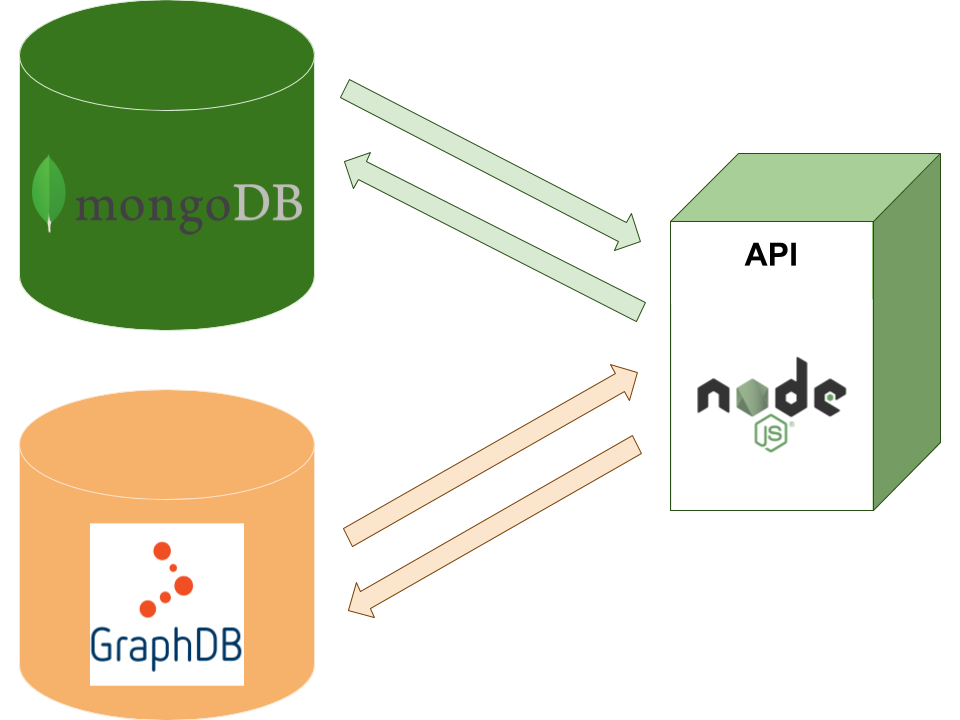
\includegraphics[width=10cm]{Pictures/backend.png}
    \caption{Estrutura do backend}
    \label{backend}
\end{figure}

Esta estrutura, demonstrada na figura acima (fig. \ref{backend}), é modular, ou seja, cada um dos três componentes identificados pode estar num servidor/máquina diferente, o que permite escalar a API.

Nas próximas secções será aprofundado os vários constituintes e camadas da API.

\subsection{Modelos}

Nos \texttt{Models} define se os \textit{schemas} das coleções de documentos da base de dados \textit{MongoDB}. Cada ficheiro \texttt{.js} corresponde a uma coleção, sendo que cada \texttt{schema} permite definir a estrutura de cada tipo de documento. Foram definidos os seguintes \textit{Schemas}/Documentos:

\paragraph{\textbf{User:}} representa um utilizador
    \begin{itemize}
        \item \texttt{name:} String obrigatória referente ao nome do utilizador;
        \item \texttt{email:} String obrigatória, única, ou seja sem repetição na base de dados, portanto pode servir de identificação, representado o email do utilizador;
        \item \texttt{password:} String obrigatória encriptada referente à password do utilizador;
        \item \texttt{stats:} lista com as estatísticas do utilizador;
            \begin{itemize}
                \item \texttt{id:} id (String) do \textit{Recording} a que se associa os valores seguintes;
                \item \texttt{views:} número de visualizações do utilizador deste \textit{Recording};
                \item \texttt{rating:} classificação dado pelo utilizador a este \textit{Recording}.
            \end{itemize}
    \end{itemize}

\paragraph{\textbf{Stats:}} salvaguarda as estatísticas que antigos utilizadores (utilizadores que apagaram a sua conta)
    \begin{itemize}
        \item \texttt{id:} id (String) do \textit{Recording} a que se associa os valores seguintes;
        \item \texttt{views:} número de visualizações do \textit{Recording} salvaguardadas;
        \item \texttt{avgRating:} classificação média do \textit{Recording} salvaguardada;
        \item \texttt{nRating:} número de utilizadores que classificaram o \textit{Recording}.
    \end{itemize}

\subsection{Controladores}

Os \texttt{controllers} possuem várias funções que permitem manusear os documentos e os seus valores. As coleções de documentos são estruturados por \texttt{Schemas} recorrendo ao \texttt{Mongoose}, sendo nos \texttt{Controllers} onde se encontram definidos a criação, atualização, destruição, listagem e obtenção de estatísticas dos mesmos. Apresentasse de seguida os \textit{controllers} dos \textit{models} \textit{User} e \textit{Stats} (quando se refere música assuma o mesmo que \textit{Recording}):

\paragraph{\textbf{User:}}
    \begin{itemize}
        \item \texttt{findOne}: Dado um email obtém a informação do utilizador com esse email associado;
        \item \texttt{getUser}: Dado um id obtém a informação do utilizador com esse id associado;
        \item \texttt{isValidPassword}: Dadas duas passwords, compara-as, verificando se são iguais;
        \item \texttt{createUser}: Dada a informação de um utilizador, encripta a password, criando, por fim, o utilizador;
        \item \texttt{updateUser}: Dada a informação a atualizar (\textit{name} e/ou \textit{email}) e o id do utilizador, atualiza a informação deste; esta função restringe o acesso, ou seja, apenas o próprio utilizador pode atualizar a sua informação;
        \item \texttt{updatePassword}: dado o id de um utilizador, a password atual e a nova password, verifica se a password atual está correta (se é igual à presente na base de dados), e em caso afirmativo, encripta a nova password e passa a ser a password atual do utilizador;
        \item \texttt{deleteUser}: dado um id de um utilizador, apaga-o;
        \item \texttt{getRecordingsUser}: dado um id de um utilizador, obtém uma lista com todas as estatisticas do utilizador (visualizações e classificações);
        \item \texttt{getMoreRecordingsViewsUser}: dado um id de um utilizador, obtém uma lista das 10 músicas mais ouvidas/vistas pelo utilizador; cada elemento desta lista tem o id da música e o número de visualizações desta;
        \item \texttt{getRecordingUserRating}: dado um id de um utilizador e um id de uma música, devolve a classificação dada pelo utilizado à música; caso o utilizador não a tenha classificado, devolve 0;
        \item \texttt{updateViews}: dado um id de um utilizador e o id de uma música, soma mais uma visualização a uma música, caso as estatísticas para essa música já existam; caso não exista cria uma, com número de visualizações igual a 1 e classificação igual a 0;
        \item \texttt{updateRating}: dado um id de um utilizador, o id de uma música e a classificação a atribuir, caso as estatítiscas para esta música ja existam, atribui a nova classificação; caso não exista cria uma nova estatística para a música, com o número de visualizações igual a 0 e a classificação igual ao que foi inserida.
    \end{itemize}

\paragraph{\textbf{Stats:}}
    \begin{itemize}
        \item \texttt{createOrUpdate}: dado estatísticas de uma música (id, \textit{views}, \textit{rating}), agrega estes valores com os existentes, caso já exista o documento para o id desta música; caso ainda não exista é criado um;
        \item \texttt{getStats}: obtém todas as estatísticas, estejam elas presentes nos documentos \textit{Stats} ou nos utilizadores;
        \item \texttt{getMoreRecordingsViews}: obtém as 10 músicas mais ouvidas;
        \item \texttt{getRecordingStats}: dado o id de uma música, obtém as estatísticas para esta música;
        \item Nota: Para obter as estatísticas, foi necessário, como já referido, aceder aos documentos dos utilizadores a partir deste \texttt{controller}.
    \end{itemize}

Por outro lado, também é aqui nos \texttt{controllers} que são realizadas as \textit{queries} à base de dados \textit{GraphDB}. Por forma, a modularizar o código, no ficheiro \textit{execQuery.js} é definida a função \texttt{execQuery}, onde apenas recebe a \textit{query} a ser realizada, e devolve o resultado já ``limpo'', ou seja, uma lista de resultados, onde cada elemento, tem como atributos as variáveis devolvidas pela \textit{query} e como valor o seu valor obtido. A função \texttt{execQuery} já inclui o prefixo da ontologia pelo que na \textit{query} não é necessário indicar a totalidade do \textit{URI} bastando apenas colocar ``:'' quando se refere a um \textit{URI} da ontologia definida neste trabalho (ver \ref{ontologia}). Todas as \textit{queries} realizadas são de leitura de informação, sendo estas dividas em ficheiros pela classe que questionam. Sendo assim existem os seguintes \texttt{controllers} que questionam o \textit{GraphDB} de forma a obter informação de indivíduos da classe:

\paragraph{\textbf{Album:}}
    \begin{itemize}
        \item \texttt{listAlbums}: dado um \textit{offset}, lista os 50 albums (id e título do album) a partir do \textit{offset} da lista ordenada (pelos títulos) de todos os albums;
        \item \texttt{listAlbumsByFilter}: dado um \textit{offset} e um filtro, devolve o mesmo que o anterior contudo em vez da lista ordenada ser de todos os albums, é apenas dos albums que começam pelo valor presente no filtro;
        \item \texttt{getAlbum}: dado o id de um album, obtém o título, e caso exista, data da primeira \textit{release}, sobre (\textit{about}) e desambiguação;
        \item \texttt{getURLs}: dado o id de um album, obtém os \textit{URLs} sobre o album, devolvendo uma lista onde cada elemento possui o nome do website e o \textit{URL};
        \item \texttt{getTracks}: dado o id de um album, obtém as músicas pertencentes ao album, devolvendo uma lista, em que cada elemento tem o id, título, duração e, caso exista, desambiguação de uma música;
        \item \texttt{getTags}: dado o id de um album, obtém as tags do album, através das tags pertencentes às músicas pertencentes ao album;
        \item \texttt{getArtistsCredit}: dado o id de um album, obtém os artistas do album através dos artistas associados às músicas pertencentes ao album.
    \end{itemize}

\paragraph{\textbf{Area:}}
    \begin{itemize}
        \item \texttt{listAreas}: dado um \textit{offset}, lista as 50 areas (id e nome da area) a partir do \textit{offset} da lista ordenada (pelos nomes) de todas os areas;
        \item \texttt{listAreasByFilter}: dado um \textit{offset} e um filtro, devolve o mesmo que o anterior contudo em vez da lista ordenada ser de todas as areas, é apenas das areas que começam pelo valor presente no filtro;
        \item \texttt{getArea}: dado o id de uma area, obtém o nome, o tipo, e caso exista, sobre (\textit{about}) e desambiguação;
        \item \texttt{getAliases}: dado o id de uma area obtém os nomes alternativos para a area;
        \item \texttt{getPartOf}: dado o id de uma area obtém o id, nome e tipo das areas a que pertence;
        \item \texttt{getParts}: dado o id de uma area obtém o id, nome e tipo das areas que contém;
        \item \texttt{getURLs}: dado o id de uma area, obtém os \textit{URLs} sobre a area, devolvendo uma lista onde cada elemento possui o nome do website e o \textit{URL};
        \item \texttt{getArtists}: dado o id de uma area, obtém os artistas que são dessa area, devolvendo para cada artista o seu id e nome.
    \end{itemize}

\paragraph{\textbf{Artist:}}
    \begin{itemize}
        \item \texttt{listArtists}: dado um \textit{offset}, lista os 50 artistas (id e nome do artista) a partir do \textit{offset} da lista ordenada (pelos nomes) de todas os artistas;
        \item \texttt{listArtistsByFilter}: dado um \textit{offset} e um filtro, devolve o mesmo que o anterior contudo em vez da lista ordenada ser de todos os artistas, é apenas dos artistas que começam pelo valor presente no filtro;
        \item \texttt{getArtist}: dado o id de um artista, obtém o nome, e caso exista, o tipo, o nome para ordenar, a data de nascimento/início, a data de falecimento/fim, o sexo, o id da area, o nome da area, sobre (\textit{about}) e desambiguação;
        \item \texttt{getAliases}: dado o id de um artista obtém os nomes alternativos para o artista;
        \item \texttt{getURLs}: dado o id de um artista, obtém os \textit{URLs} sobre o artista, devolvendo uma lista onde cada elemento possui o nome do website e o \textit{URL};
        \item \texttt{getRecordings}: dado o id de um artista, devolve o id e o título das músicas no qual o artista fez parte;
        \item \texttt{getTags}: dado o id de um artista, obtém as tags do artista, através das tags pertencentes às músicas no qual o artista fez parte;
        \item \texttt{getAlbums}: dado o id de um artista, obtém os albums do artista onde o artista possui músicas nas quais fez parte.
    \end{itemize}

\paragraph{\textbf{Recording:}}
    \begin{itemize}
        \item \texttt{listRecordings}: dado um \textit{offset}, lista as 50 músicas (id e título da música) a partir do \textit{offset} da lista ordenada (pelos títulos) de todas as músicas;
        \item \texttt{listRecordingsByFilter}: dado um \textit{offset} e um filtro, devolve o mesmo que o anterior contudo em vez da lista ordenada ser de todas as músicas, é apenas das músicas que começam pelo valor presente no filtro;
        \item \texttt{getRecording}: dado o id de uma música, obtém o título, e caso exista, a duração, sobre (\textit{about}) e desambiguação;
        \item \texttt{getLanguages}: dado o id de uma música obtém as línguas usadas;
        \item \texttt{getTags}: dado o id de uma música, obtém as tags da música;
        \item \texttt{getURLs}: dado o id de uma música, obtém os \textit{URLs} sobre a música, devolvendo uma lista onde cada elemento possui o nome do website e o \textit{URL};
        \item \texttt{getArtistsCredit}: dado o id de uma música, devolve o id e o nome dos artistas que fizeram parte da música;
        \item \texttt{getAlbums}: dado o id de uma música, devolve os albums no qual a música faz parte;
        \item \texttt{searchForRecordings}: dados dois filtros, um para o nome de um artista e outro para um título de uma música, obtém o id, nome do artista e título de músicas em que o nome do artista comece pelo seu filtro e o título da música comece também pelo seu filtro.
    \end{itemize}

\subsection{Rotas}

As rotas encaminham os pedidos dos clientes de forma a realizarem a correta chamada de funções presentes nos \texttt{Controllers}, sendo que a rota para onde o utilizador é encaminhado varia consoante o \texttt{URL} e o método do pedido.
De seguida, apresentam-se as rotas, a função que é chamada para cada rota e é referido alguns passos adicionais que são realizados em alguns casos.

\paragraph{\textit{Controller} User: rota \texttt{/users} concatenada com:}
    \begin{itemize}
        \item método \texttt{GET}
            \begin{itemize}
                \item \texttt{/isAuthenticated} - devolve ``Authenticated'' se o utilizador estiver autenticado, caso contrário devolve ``Unauthorized'', permite saber se um utilizador está autenticado
                \item \texttt{/:id/statsMore} - \texttt{getMoreRecordingsViewsUser(:id)} se o ``:id'' for igual ao id do utilizador que está autenticado, senão devolve uma mensagem de erro
                \item \texttt{/:id/stats?idRec=idRecI} - \texttt{getRecordingUserRating(:id, idRecI)} se o ``:id'' for igual ao id do utilizador que está autenticado, senão devolve uma mensagem de erro
                \item \texttt{/:id/stats} - \texttt{getRecordingsUser(:id)} se o ``:id'' for igual ao id do utilizador que está autenticado, senão devolve uma mensagem de erro
                \item \texttt{/:id} - \texttt{getUser(:id)} se o ``:id'' for igual ao id do utilizador que está autenticado, senão devolve uma mensagem de erro
            \end{itemize}
        \item método \texttt{POST}
            \begin{itemize}
                \item \texttt{/login} - permite a autenticação de um utilizador, caso o utilizador exista e a password seja a correta, é gerado um \textit{token} que é enviado ao cliente, esta parte será vista mais à frente (ver \ref{auth}) 
                \item \texttt{/} - \texttt{createUser(body)}
            \end{itemize}
        \item método \texttt{PUT}
            \begin{itemize}
                \item \texttt{/views/:id} - \texttt{updateViews(:id, body.idMusic)} se o ``:id'' for igual ao id do utilizador que está autenticado, senão devolve uma mensagem de erro
                \item \texttt{/rating/:id} - \texttt{updateRating(:id, body.idMusic, body.rating)} se o ``:id'' for igual ao id do utilizador que está autenticado, senão devolve uma mensagem de erro
                \item \texttt{/updPass/:id} - \texttt{updatePassword(:id, body.prevPass, body.newPass)} se o ``:id'' for igual ao id do utilizador que está autenticado, senão devolve uma mensagem de erro
                \item \texttt{/:id} - \texttt{updateUser(:id, body)} se o ``:id'' for igual ao id do utilizador que está autenticado, senão devolve uma mensagem de erro
            \end{itemize}
        \item método \texttt{DELETE}
            \begin{itemize}
                \item \texttt{/:id} - \texttt{deleteUser(:id)} e para cada sub documento de estatísticas do utilizador apagado (\texttt{stat}) é realizado \texttt{createOrUpdate(stat)} do \texttt{controller} Stats, se o ``:id'' for igual ao id do utilizador que está autenticado, senão devolve uma mensagem de erro
            \end{itemize}
    \end{itemize}

\paragraph{\textit{Controller} Stats: rota \texttt{/stats} concatenada com:}
    \begin{itemize}
        \item método \texttt{GET}
            \begin{itemize}
                \item \texttt{/more} - \texttt{getMoreRecordingsViews()} 
                \item \texttt{/:id} - \texttt{getRecordingStats(:id)} 
                \item \texttt{/} - \texttt{getStats()} 
            \end{itemize}
        \item método \texttt{POST}
            \begin{itemize}
                \item \texttt{/} - \texttt{createOrUpdate(body)}
            \end{itemize}
    \end{itemize}

\paragraph{\textit{Controller} Album: rota \texttt{/albums} concatenada com:}
    \begin{itemize}
        \item método \texttt{GET}
            \begin{itemize}
                \item \texttt{/:id/tags} - \texttt{getTags(:id)} 
                \item \texttt{/:id/tracks} - \texttt{getTracks(:id)} 
                \item \texttt{/:id/artistsCredit} - \texttt{getArtistsCredit(:id)} 
                \item \texttt{/:id/urls} - \texttt{getURLs(:id)} 
                \item \texttt{/:id} - \texttt{getAlbum(:id)} 
                \item \texttt{?offset=offsetI\&filter=filterI} - \texttt{listAlbumsByFilter(offsetI, filterI)}
                \item \texttt{?filter=filterI} - \texttt{listAlbumsByFilter(0, filterI)}
                \item \texttt{?offset=offsetI} - \texttt{listAlbums(offsetI)}
                \item \texttt{/} - \texttt{listAlbums(0)}
            \end{itemize}
    \end{itemize}

\paragraph{\textit{Controller} Area: rota \texttt{/areas} concatenada com:}
    \begin{itemize}
        \item método \texttt{GET}
            \begin{itemize}
                \item \texttt{/:id/aliases} - \texttt{getAliases(:id)}
                \item \texttt{/:id/artists} - \texttt{getArtists(:id)}
                \item \texttt{/:id/urls} - \texttt{getURLs(:id)}
                \item \texttt{/:id/parts} - \texttt{getParts(:id)}
                \item \texttt{/:id/partOf} - \texttt{getPartOf(:id)}
                \item \texttt{/:id} - \texttt{getArea(:id)}
                \item \texttt{?offset=offsetI\&filter=filterI} - \texttt{listAreasByFilter(offsetI, filterI)}
                \item \texttt{?filter=filterI} - \texttt{listAreasByFilter(0, filterI)}
                \item \texttt{?offset=offsetI} - \texttt{listAreas(offsetI)}
                \item \texttt{/} - \texttt{listAreas(0)}
            \end{itemize}
    \end{itemize}

\paragraph{\textit{Controller} Artist: rota \texttt{/artists} concatenada com:}
    \begin{itemize}
        \item método \texttt{GET}
            \begin{itemize}
                \item \texttt{/:id/tags} -  \texttt{getTags(:id)}
                \item \texttt{/:id/albums} - \texttt{getAlbums(:id)}
                \item \texttt{/:id/recordings} - \texttt{getRecordings(:id)}
                \item \texttt{/:id/urls} - \texttt{getURLs(:id)}
                \item \texttt{/:id/aliases} - \texttt{getAliases(:id)}
                \item \texttt{/:id} - \texttt{getArtist(:id)}
                \item \texttt{?offset=offsetI\&filter=filterI} - \texttt{listArtistsByFilter(offsetI, filterI)}
                \item \texttt{?filter=filterI} - \texttt{listArtistsByFilter(0, filterI)}
                \item \texttt{?offset=offsetI} - \texttt{listArtists(offsetI)}
                \item \texttt{/} - \texttt{listArtists(0)}
            \end{itemize}
    \end{itemize}

\paragraph{\textit{Controller} Recording: rota \texttt{/recordings} concatenada com:}
    \begin{itemize}
        \item método \texttt{GET}
            \begin{itemize}
                \item \texttt{/search?name=nameI\&title=titleI} - \texttt{searchForRecordings(nameI, titleI)}
                \item \texttt{/:id/albums} - \texttt{getAlbums(:id)}
                \item \texttt{/:id/artistsCredit} - \texttt{getArtistsCredit(:id)}
                \item \texttt{/:id/urls} - \texttt{getURLs(:id)}
                \item \texttt{/:id/languages} - \texttt{getLanguages(:id)}
                \item \texttt{/:id/tags} - \texttt{getTags(:id)}
                \item \texttt{/:id} - \texttt{getRecording(:id)}
                \item \texttt{?offset=offsetI\&filter=filterI} - \texttt{listRecordingsByFilter(offsetI, filterI)}
                \item \texttt{?filter=filterI} - \texttt{listRecordingsByFilter(0, filterI)}
                \item \texttt{?offset=offsetI} - \texttt{listRecordings(offsetI)}
                \item \texttt{/} - \texttt{listRecordings(0)}
            \end{itemize}
    \end{itemize}

\subsection{Autenticação} \label{auth}

As rotas da API estão quase todas protegidas à exceção de duas, \texttt{GET} de \texttt{/users/login} e \texttt{POST} de \texttt{/users}. A primeira rota não está protegida porque é onde os utilizadores podem realizar \textit{login}, e que em caso de autenticação com sucesso é gerado um \texttt{token} que é enviado para o utilizador. Já a segunda rota permite a criação (registo) de utilizadores.

De forma a aceder às rotas protegidas, os clientes tem de enviar o \texttt{token}, que lhes foi fornecido, nas \texttt{headers} do pedido, mais precisamente na \textit{header} \texttt{Authorization}, sendo o valor a colocar neste campo igual a \texttt{Bearer \$\{token\}}.

\begin{figure}[H]
    \centering
    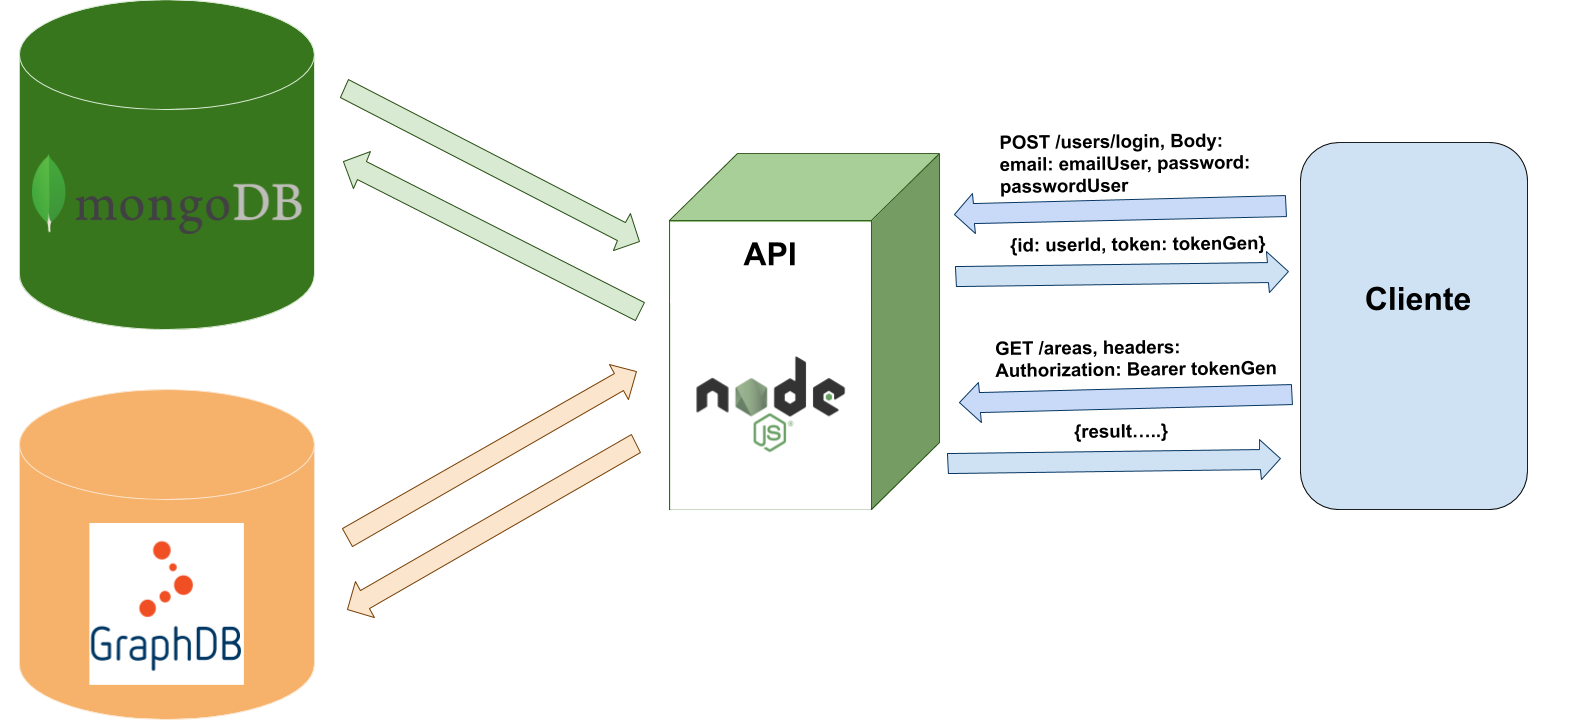
\includegraphics[width=15cm]{Pictures/exeAuth.png}
    \caption{Um exemplo de um login e posterior pedido com envio do \textit{token}}
    \label{exe_auth}
\end{figure}

O \textit{token} tem um tempo de validade, pelo que ao fim de 30 minutos expira.
A autenticação é realizada com a ajuda do \texttt{passport-local}. De forma a gerar o \textit{token} recorre-se ao \texttt{jsonwebtoken} usando uma chave privada para gerar o \textit{token} através do algoritmo RS256 (\textit{RSA Signature with SHA-256}). Já na verificação do \textit{token} é utilizado o \texttt{passport-jwt} com a tática de extração \texttt{fromAuthHeaderAsBearerToken}, daí a necessidade de colocar o \textit{token} nas headers dos pedidos como indicado. Esta verificação recorre à chave pública para confirmar a validade do \textit{token}.

\section{Interface}

A interface foi desenvolvida através da \textit{framework} \texttt{Vue.js} e a \textit{framework} de material \texttt{Vuetify.js} baseada no \textit{Material Design} da \textit{Google}. Esta interface estará no lado do utilizador, enquanto que a API está presente num servidor. Claro, contudo, esta interface tem de ser armazenada num servidor, de forma aos clientes/utilizadores fazerem o download desta interface, para posteriormente acederem diretamente à API através da interface.

Quanto a imagens usadas na interface, estas estão armazenadas em \texttt{public/static/}.

\begin{figure}[H]
    \centering
    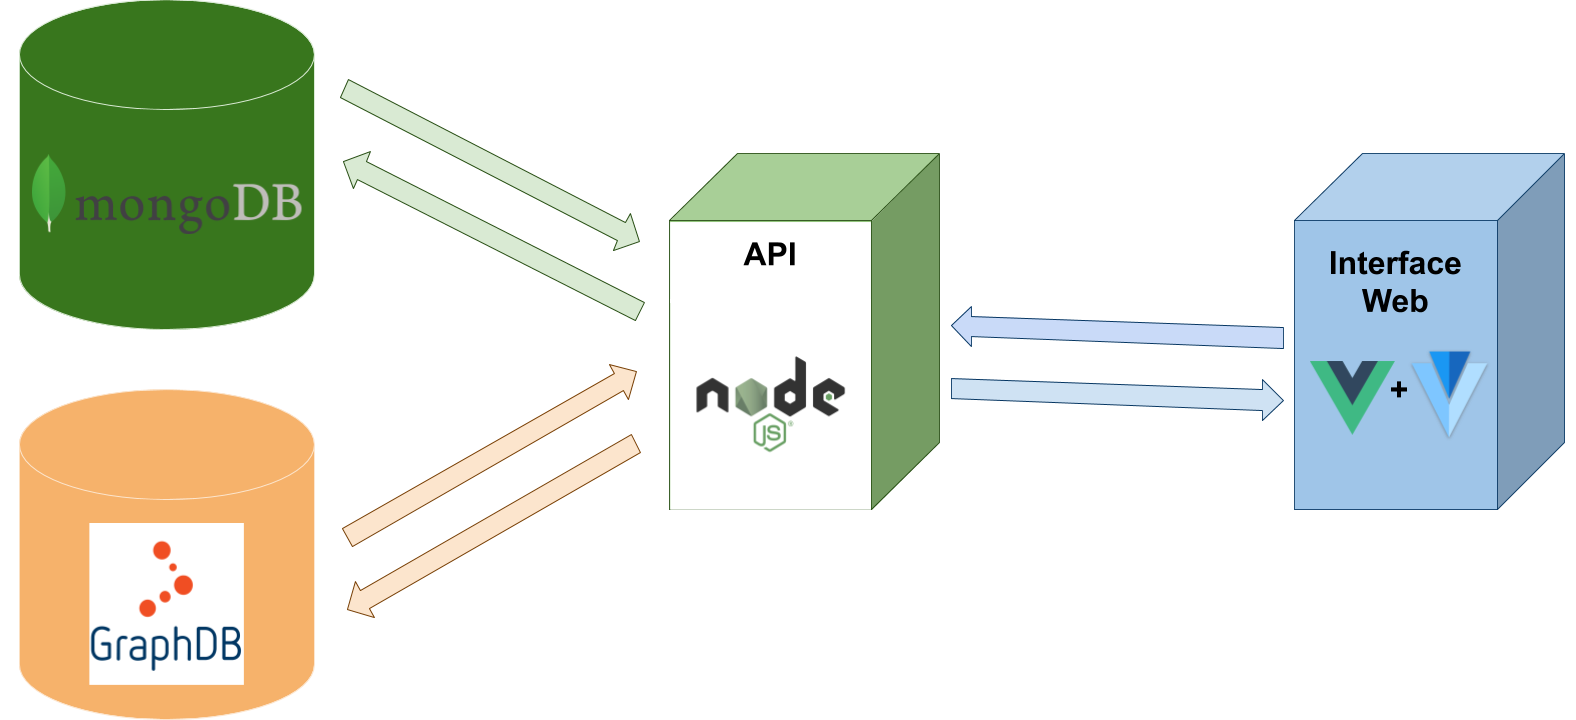
\includegraphics[width=12cm]{Pictures/backend_frontend.png}
    \caption{Estrutura do backend e frontend}
    \label{backend_frontend}
\end{figure}

Já em relação ao aspeto visual da interface, ela possui um \textit{footer}, que aparece em todas as páginas, e como tal, foi definida na \texttt{App.vue}. Este \textit{footer} possui allguns \textit{URLs} importantes, desde API usadas, ao \textit{URL} onde se pode verificar o código produzido.

Já na \texttt{main.js} é definida uma variável global (\texttt{\$urlAPI}) onde está presente o \textit{URL} da API, de forma a tornar o código mais limpo e mais fácil de futuramente ser mantido. É também aqui importado uma \textit{package} \textit{wrapper} da API do \textit{iframe} do \textit{Youtube}.

De seguida, serão apresentadas as várias camadas da interface.

\subsection{Rotas}

Visto que foi usada um versão do \textit{Vue.js} com um \textit{router} existem rotas a definir, indicando para que vista as mesmas redirecionam. Apresenta-se, de seguida, as rotas definidas (presentes no ficheiro \textit{router.js}):

\begin{itemize}
    \item Rota \texttt{/recordingsSearch} $\to$ vista \texttt{RecordingsSearch.vue}
    \item Rota \texttt{/recordings/:id} $\to$ vista \texttt{Recording.vue}
    \item Rota \texttt{/areas/:id} $\to$ vista \texttt{Area.vue}
    \item Rota \texttt{/artists/:id} $\to$ vista \texttt{Artist.vue}
    \item Rota \texttt{/albums/:id} $\to$ vista \texttt{Album.vue}
    \item Rota \texttt{/userSettings/:id} $\to$ vista \texttt{UserSettings.vue}
    \item Rota \texttt{/recordings} $\to$ vista \texttt{Recordings.vue}
    \item Rota \texttt{/areas} $\to$ vista \texttt{Areas.vue}
    \item Rota \texttt{/artists} $\to$ vista \texttt{Artists.vue}
    \item Rota \texttt{/albums} $\to$ vista \texttt{Albums.vue}
    \item Rota \texttt{/index} $\to$ vista \texttt{Index.vue}
    \item Rota \texttt{/signup} $\to$ vista \texttt{SignUp.vue}
    \item Rota \texttt{/} $\to$ vista \texttt{Login.vue}
\end{itemize}

\subsection{Vistas}

As vistas definidas são bastante parecidas umas com as outras, tendo apenas algumas pequenas diferenças. 

Todas as vistas importam o componente com o mesmo nome que a vista, ou seja, por exemplo a vista \texttt{Areas.vue} importa o componente \texttt{Areas.vue}.

As vistas \texttt{Index.vue}, \texttt{Recordings.vue}, \texttt{Areas.vue}, \texttt{Artists.vue}, \texttt{Albums.vue}, \texttt{RecordingsSearch.vue}, \texttt{Recording.vue}, \texttt{Area.vue}, \texttt{Artist.vue}, \texttt{Album.vue} e \texttt{UserSettings.vue} verificam se o utilizador está autenticado, em caso afirmativo é feito a renderização da páginas; em caso negativo o utilizador é redirecionado para a página de \textit{login} (rota \texttt{/}).

Em adição, as vistas \texttt{Recording.vue}, \texttt{Area.vue}, \texttt{Artist.vue} e \texttt{Album.vue}, passam um argumento para o componente. Este argumento é o id do individuo (\textit{Recording}, \textit{Area}, \textit{Artist} ou \textit{Album} respetivamente). A vista \texttt{UserSettings.vue} também passa um argumento para o componente, contudo este argumento é o id do utilizador.

Por fim, as vistas \texttt{Login.vue} e \texttt{SignUp.vue} verificam se o utilizador está autenticado, em caso afirmativo é redirecionado para a página inicial (vista \texttt{Index.vue}, rota \texttt{/index}); em caso negativo a página é renderizada.

\subsection{Componentes}

Os componentes permitem a modularização das páginas web, fomentando uma melhor codificação.

Visto existirem várias funções que são usadas em vários componentes, foram criados os seguintes ficheiros:

\paragraph{\texttt{auth.js}:}\mbox{}\\

Possui duas funções, \texttt{isAuthenticated} e \textit{logout}. A primeira, pergunta à API se o utilizador está autenticado, caso não esteja, apaga da \textit{local storage} o \textit{token} e o id do utilizador. Já o \textit{logout} apaga da \textit{local storage} o \textit{token} e o id do utilizador, sem verificar se ainda está autenticado.

\paragraph{\texttt{request.js}:}\mbox{}\\

Este ficheiro foi criado de forma a possuir funções que simplifiquem o uso da \textit{package} \texttt{axios}, com a colocação em cabeçalho do \textit{token} do utilizador. Neste ficheiro está presente três funções, \textit{getAPI}, \textit{putAPI} e \textit{deleteAPI}. A função \textit{getAPI} recebe como argumento um \textit{url} para onde é feito um pedido \texttt{GET}. Já a função para além de um \textit{url}, recebe também dados a enviar como argumento, realizando um pedido \texttt{PUT} desses dados para o \textit{url} fornecido. Por fim, o \textit{deleteAPI} recebe como argumento um \textit{url} para onde é feito um pedido \texttt{DELETE}. Como já referido estas três funções colocam nas \textit{headers} o \textit{token} do utilizador da forma já descrita na secção \ref{auth}.

\vspace{10px}

De seguida apresentam-se os componentes criados.

\paragraph{\texttt{Login.vue}:}\mbox{}\\

Página onde se realiza o login, possui um formulário para preencher o email e a password. Possui ainda dois botões, um para autenticar e outro para ser redirecionado para a página de registo.

\paragraph{\texttt{SignUp.vue}:}\mbox{}\\

Página onde os utilizadores podem se registar. Possui um formulário, onde o utilizador necessita de indicar nome, email, password, repetir a password e depois de tudo ser validado (de forma a validar foi usado \texttt{vuelidate}) o botão para submeter o registo fica disponível. Quando o utilizador carregar, é redirecionado para a página de login, sendo mostrado uma mensagem de sucesso se o registo for efetuado com sucesso, ou pelo contrário se não tiver sucesso, aparece uma mensagem de erro.

\paragraph{\texttt{Toolbar.vue}:}\mbox{}\\

Componente usado por quase todos os componentes, com a exceção dos componentes \texttt{Login.vue} e \texttt{SignUp.vue}. Este componente representa a barra de ferramentas superior que se encontra em grande parte das páginas. Nesta barra está presente vários links para diferentes páginas da interface, o primeiro onde está o nome da aplicação e o seu símbolo, redireciona para a página inicial (\texttt{/index}). Depois por ordem, links para listagem de \textit{Albums}, \textit{Recordings}, \textit{Artists} e \textit{Areas}, para a página de configuração do utilizador e por fim \textit{Logout}. Quando o utilizador está numa destas páginas, a barra de ferramentas sinaliza a mesma ao usar uma cor diferente para o botão associada a essa página.

Para além disso, esta barra, por vezes, apresenta uma caixa de texto por forma filtrar os resultados disponíveis ou para pesquisar. Quando se está nas páginas de listagem de \textit{Albums}, \textit{Recordings}, \textit{Artists} e \textit{Areas} esta caixa de texto permite filtrar os resultados. Nas restantes páginas em que aparece (página de um individuo \textit{Album}, \textit{Recording}, \textit{Artist} ou \textit{Area} e na página inicial \textit{Index}), esta caixa de texto permite pesquisar por arista mais música com o formato ``\textit{Artist}-\textit{Recording}.

\paragraph{\texttt{Index.vue}:}\mbox{}\\

Página inicial da interface. Apresenta estatísticas do utilizador e da aplicação, como as músicas mais ouvidas, entre outras (ver \ref{tema}). Ao carregar numa das músicas, albums, artistas ou areas, o utilizador é redirecionado para a página desse individuo.

\paragraph{\texttt{Albums.vue}:}\mbox{}\\

Lista todos os albums, mas por partes de 50 albums, devido à grande quantidade de albums. Ao fim dos 50 albums, apresenta-se um botão, de forma a obter os próximos 50 albums. Todos os albums renderizados, são clicáveis de forma a obter mais informação (redirecionamento para a página do album).

\paragraph{\texttt{Areas.vue}:}\mbox{}\\

Lista todos os areas, mas por partes de 50 areas, devido à grande quantidade de areas. Ao fim das 50 areas, apresenta-se um botão, de forma a obter as próximas 50 areas. Todas as areas renderizadas, são clicáveis de forma a obter mais informação (redirecionamento para a página da area).

\paragraph{\texttt{Artists.vue}:}\mbox{}\\

Lista todos os artistas, mas por partes de 50 artistas, devido à grande quantidade de artistas. Ao fim dos 50 artistas, apresenta-se um botão, de forma a obter os próximos 50 artistas. Todos os artistas renderizados, são clicáveis de forma a obter mais informação (redirecionamento para a página do artista).

\paragraph{\texttt{Recordings.vue}:}\mbox{}\\

Lista todos as músicas, mas por partes de 50 músicas, devido à grande quantidade de músicas. Ao fim das 50 músicas, apresenta-se um botão, de forma a obter as próximas 50 músicas. Todas as músicas renderizadas, são clicáveis de forma a obter mais informação (redirecionamento para a página da música).

\paragraph{\texttt{RecordingsSearch.vue}:}\mbox{}\\

Página para onde o utilizador é redirecionado quando pesquisa na caixa de texto com o formato ``\textit{Artist}-\textit{Recording}''. Lista as músicas que obedecem à pesquisa, sendo possível obter mais informação da música ao clicar nela (o utilizador é redirecionado para a página da música).

\paragraph{\texttt{Album.vue}:}\mbox{}\\

Página que apresenta toda a informação de um determinado individuo da classe \textit{Album}. Apresenta também a classificação e o rating do album. (ver \ref{tema})

\paragraph{\texttt{Area.vue}:}\mbox{}\\

Página que apresenta toda a informação de um determinado individuo da classe \textit{Area}. (ver \ref{tema})

\paragraph{\texttt{Artist.vue}:}\mbox{}\\

Página que apresenta toda a informação de um determinado individuo da classe \textit{Artist}. Apresenta também a classificação e o rating do artista. (ver \ref{tema})

\paragraph{\texttt{Recording.vue}:}\mbox{}\\

Página que apresenta toda a informação de um determinado individuo da classe \textit{Recording}. Apresenta também a classificação e o rating da música. Para além disso mostra o vídeo da música (quando possível, nem sempre acerta no vídeo correto) e as \textit{lyrics} da música. As \textit{lyrics} da música são obtidas a partid de duas APIs diferentes, \textit{musixmatch} e \textit{Chartlyrics}. (ver \ref{tema})

\paragraph{\texttt{UserSettings.vue}:}\mbox{}\\

Nesta página, estão presentes dois formulários onde o utilizador pode, num deles atualizar a sua password e no outro atualizar a sua informação (nome e email).

\paragraph{\texttt{Youtube.vue}:}\mbox{}\\

Componente usado pela página onde se apresenta um individuo da classe \textit{Recording}. Permite pesquisar vídeos do \textit{YouTube} por uma \textit{string} e mostrar o vídeo que mais se associa.

\section{Instalação}

~\cite{mbAnnotation}

\section{Conclusões e Trabalho Futuro}

%tornar queries mais rápidas, as que são lentas, adicionar paginação nas listagems, criação e gestão de playlists, sugestão de músicas ao utilizador. As estatísticas 'paises com mais artistas', 'paises com mais músicas' e 'paises com mais albuns' não foram realizadas visto que atuais queries que varrem apenas uma das entidades demoram pelo menos 10 segundos, estas seriam ainda mais lentas

\newpage 
\printbibliography

\begin{appendices}

\end{appendices}

\end{document}
